\subsection{Level \texorpdfstring{$\alpha$}{alpha} Tests: General Approach}
\label{subsec:level-alpha-tests}

A standard algorithm for a level $\alpha$ test of a hypothesis $H_0$ against an alternative $H_A$ consists of 3 steps.

\subsubsection*{Step 1. Test Statistic}

Testing hypothesis is based on a \textbf{test statistic} $T$ , a quantity computed from the data that has some known, tabulated distribution $F_0$ if the hypothesis $H_0$ is true.

\subsubsection*{Step 2. Acceptance Region and Rejection Region}

Next, we consider the \textbf{null distribution} $F_0$. This is the distribution of test statistic $T$ when the hypothesis $H_0$ is true. If it has a density $f_0$, then the whole area under the density curve is 1, and we can always find a portion of it whose area is $\alpha$, as shown in Figure 5. It is called \textbf{rejection region} ($\mathcal{R}$).

The remaining part, the complement of the rejection region, is called \textbf{acceptance region} ($\mathcal{A = \overline{R}}$). By the complement rule, its area is ($1 - \alpha$).

\subsubsection*{Step 3. Result and Its Interpretation}

Accept the hypothesis $H_0$ if the test statistic $T$ belongs to the acceptance region. Reject $H_0$ in favor of the alternative $H_A$ if $T$ belongs to the rejection region.

\begin{figure}[H]
  \centering
  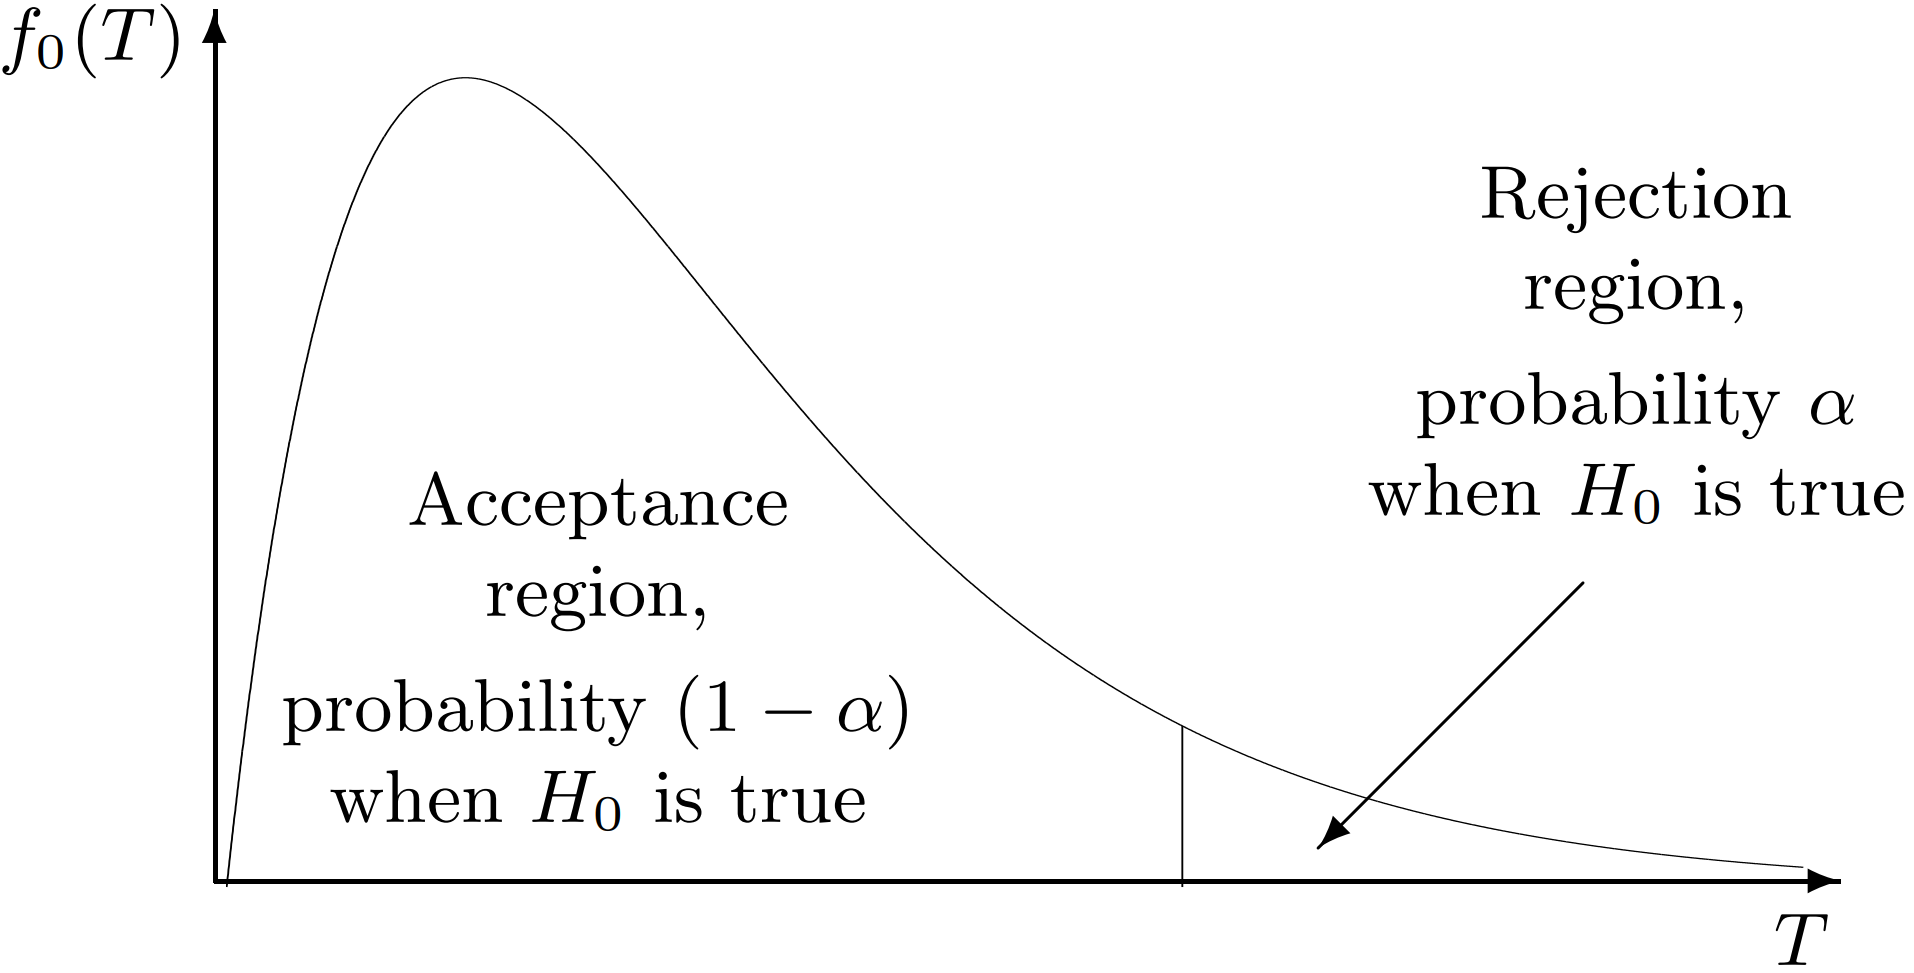
\includegraphics[width=\linewidth]{img/fig-9.6.png}
  \caption{}
  \label{fig:9.6}
\end{figure}
